\section{Experiments}
\label{sec:experiments}

% Talk about Epochs
% Talk about the different experiments
% Talk about the different measures

All experiments are controlled by an \texttt{ExperimentManager} which is responsible for the following tasks:
\begin{itemize}
    \item Create the \texttt{Infrastructure}, which consists of \texttt{Node}s, \texttt{Agent}s, and \texttt{Software Component}s.
    \item Attach event listeners to \texttt{Node}s and \texttt{Agent}s to measure (depending on the experiment) for example the number of adaptations, the number of messages exchanged, and the number of risks identified.
    \item Send custom events \texttt{Agent}s.
    \item Keep track of the current epoch and stop the experiment after a predefined number of epochs.
\end{itemize}

\subsection{Baseline Experiment}
% - No communication, no cooperation
% - Predefined Infrastructure, same as other experiments
% - Measure:
%   - Number of adaptations
%   - Total number of risks identified
%   - Number of remaining risks
%   - Sum of the damage for remaining risks

% Mitigations take time, also communication. This should be discussed and used in the experiment.
% Check costs of a mitigation

\begin{itemize}
    \item The agents are still connected to the \texttt{ExperimentManager} but do not communicate with each other. This is done to be able to mimic and measure events.
    \item Agents are allowed to adapt their own properties and software components.
    \item Agents are not allowed to adapt the properties and software components of other agents/nodes.
\end{itemize}

\begin{figure}[H]
    \centering
    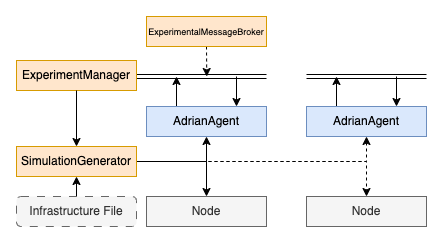
\includegraphics[width=0.8\textwidth]{_content/adrian-experiment-0}
    \caption{Baseline experiment}
    \label{fig:baseline}
\end{figure}

\subsection{Experiment 1: Risk Analysis (communication)}
% - Communication, no cooperation
% - Predefined Infrastructure, same as other experiments
% - Measure:
%   - Number of adaptations
%   - Total number of messages exchanged
%   - Total number of risks identified
%   - Number of remaining risks
%   - Sum of the damage for remaining risks

\begin{figure}[H]
    \centering
    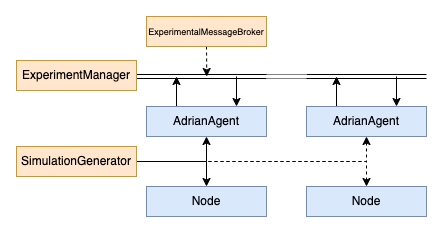
\includegraphics[width=0.8\textwidth]{_content/adrian-experiment-1}
    \caption{Experiment 1: Risk Analysis (communication)}
    \label{fig:experiment-1}
\end{figure}

\subsection{Experiment 2: Risk Mitigation (cooperation)}
% - Communication, cooperation
% - Predefined Infrastructure, same as other experiments
% - Measure:
%   - Number of adaptations
%   - Total number of messages exchanged
%   - Total number of risks identified
%   - Number of remaining risks
%   - Sum of the damage for remaining risks

